\documentclass[technicalreport]{ieicej}
%\documentclass[technicalreport,usejistfm]{ieicej}
\usepackage[dvipdfmx]{graphicx}
\usepackage{latexsym}
%\usepackage[fleqn]{amsmath}
\usepackage{amsmath}
\usepackage{amssymb}
\usepackage{multirow,eepic}
\usepackage{cite}
\usepackage{mediabb}
\usepackage{url}
\usepackage{comment}
\usepackage{epsfig}
\usepackage{subfig}
\setlength{\oddsidemargin}{-9mm}
\setlength{\evensidemargin}{-9mm}
\setlength{\topmargin}{-4mm}
%\renewcommand{\topfraction}{1.0}
%\renewcommand{\bottomfraction}{1.0}
%\renewcommand{\dbltopfraction}{1.0}
%\renewcommand{\textfraction}{0.01}
%\renewcommand{\floatpagefraction}{1.0}
%\renewcommand{\dblfloatpagefraction}{1.0}
\setcounter{topnumber}{5}
\setcounter{bottomnumber}{5}
\setcounter{totalnumber}{10}

\newcommand{\sij}{(i,\ j)}
\newcommand{\mN}{{\mathcal N}}
\newcommand{\pij}{p^{(i,\ j)}}
\newcommand{\rd}{r^{\sij}_{\rm d}}
\newcommand{\ru}{r^{\sij}_{\rm u}}
\newcommand{\rij}{r^{\sij}}
\newcommand{\etau}{\eta_{\rm u}^{(j)}}

\jtitle{QoS向上に向けた送信機会の最適化}
%\jsubtitle{}
\etitle{Transmission Opportunity Optimization for QoS improvement}
%\esubtitle{}
 \alignorder=4
 \breakauthorline{4}

\authorlist{%
 \authorentry[info16@imc.cce.i.kyoto-u.ac.jp]{飯田 直人}{Naoto Iida}{^1}
 \authorentry{西尾 理志}{Takayuki NISHIO}{^1}
 \authorentry{守倉 正博}{Masahiro MORIKURA}{^1}
 \authorentry{山本 高至}{Koji YAMAMOTO}{^1}
 \authorentry{鍋谷 寿久}{Toshihisa Nabetani}{^2}
 \authorentry{青木 亜秀}{Tsuguhide Aoki}{^2}
 }

\affiliate[^1]{京都大学 大学院情報学研究科\hskip1zw
  〒606-8501 京都市左京区吉田本町}
 {Graduate School of Informatics, Kyoto University\hskip1em
  Yoshida-honmachi, Sakyo-ku, Kyoto,
  606-8501 Japan}
\affiliate[^2]{株式会社東芝 研究開発センター\hskip 1zw 〒212-8582 神奈川県川崎市幸区小向東芝町1}
  {Corporate Research \& Development Center, TOSHIBA Corporation\hskip1em
   1 Komukaitoshiba-cho, Saiwai-ku, Kawasaki-shi, Kanagawa 212-8582, Japan}

\begin{document}
\begin{jabstract}
	全二重通信無線LANでは送信と受信を同時に同じ周波数帯で行うため,
	1台のAP(Access Point)と2台のSTA(station)による一方向全二重通信の場合,
	APの所望信号に自身の送信信号が影響を与える自己干渉と,
	STAの送信信号が別のSTAの受信信号に干渉を与えるユーザ間干渉が問題となる.
	自己干渉は自己干渉除去技術によって低減可能であるが,ユーザ間干渉は除去できない.
	そのため,ユーザ間干渉の影響を小さくするため,全二重通信を参加する2台のSTAの組み合わせをユーザ間干渉を考慮して決定する手法が検討されている.
	しかし,それらの手法では自己干渉やユーザ間干渉の量に応じて変動する過去の受信成功確率やスループットによってSTAの組み合わせが決定されるため,
	STA間の公平性やアプリケーションの要求の違いを考慮できていない.
	特に,遅延が小さいことが望ましいアプリケーションを用いているSTAであっても,干渉が大きければ送信機会を得にくくなる.
	本稿ではこの問題解決のために,まず,STA間での公平性を改善する.
	さらに,遅延が小さいことが望ましいアプリケーションを用いているSTAの送信機会を増加させ,QoS(Quality of Service)を向上させる手法を提案する.
	さらに,提案手法による公平性の改善効果と低遅延を要求するSTAのQoSの向上効果を計算機シミュレーションを用いて示す.
\end{jabstract}
\begin{jkeyword}
全二重通信無線LAN,ユーザ間干渉,最適化
\end{jkeyword}
\begin{eabstract}
	In in-band full-duplex wireless local area networks (WLANs), wireless devices can transmit and receive at the same time and the same frequency channel.
	Particularly in uni-directional full-duplex WLANs by one access point (AP) and two stations (STAs), self-interference and inter-user interference become a big problem.
	The self-interference is a interference in the desired signal of AP by own transmission signal, and the inter-user interference is a interference in one of the two STAs from the other STA.
	The self-interference can be canceled, but the inter-user interference cannot be canceld.
	Some authers had already proposed schemes to select the two STAs to communicate in the full-duplex system considering influences of the inter-user interferences.
	However, since these shcemes select STAs based on only the past full-duplex transmission success probability or throughput, they cannot take into account fairness between STAs and application requests like need short delay time.
	In this paper, we propose a scheme to improve the fairness and transmission opportunity optimization for quality of service (QoS) improvemnt.
	The simulation results show that the proposed methods improve the fairness and QoS.

\end{eabstract}
\begin{ekeyword}
full-duplex wireless LAN, inter-user interference, optimization
\end{ekeyword}

\maketitle

\section{はじめに}
	近年,無線LAN(Local Area Network)が急速に普及し,急増するトラヒックにより2.4\,GHz帯は逼迫しており,
	近い将来5\,GHz帯も同様の状態になることで, スループットの低下が問題となる.
	そのような状況において,無線LANシステムの大容量化が望まれる.
	大容量化を実現する方法の一つとして,送信と受信を同時に同じ周波数帯で行う全二重通信無線LANが有望である.
	全二重通信無線LANでは送信と受信を同時に同じ周波数帯で行うため,理想的には周波数利用効率を2倍にすることができる.
	この全二重通信無線LANの実現に向けては様々なMAC(Media Access Control)プロトコルが提案されている~\cite{fdmac, goyal, janus, fdmac2, morif, fdmac3, fcts}.
	\par
	全二重通信無線LANでは図\ref{fig:topology}に示すような従来の半二重通信では存在しなかった二つの干渉が問題となる.
	一つは,送受信を行っているAP(Access Point)において,送信信号が所望の受信信号に干渉を及ぼす自己干渉であり,
	もう一つは,STA(station)の送信信号がもう一方のSTAの受信信号に干渉を及ぼすユーザ間干渉である.
	自己干渉は自己干渉キャンセル技術によって無視できるレベルまで削減できることが示されている~\cite{fdmac, stanford1}.
	また,ユーザ間干渉に関しても,適切なSTAの組み合わせを選び出したり,
	送信電力制御を行ったりすることでユーザ間干渉を削減する手法が提案されている~\cite{contra, promac}.
	しかし,~\cite{contra}ではSTAの組み合わせを選び出すために過去の全二重通信の成功確率が用いられるため,
	干渉の影響のみが考慮されSTA間の公平性が低下する問題がある.
	また~\cite{promac}ではSTAの組み合わせの決定に際してCSMA/CA(Carrier Sence Multiple Access with Collision Avoidance)のバックオフアルゴリズムを用いるためある程度の公平性は保証されるが,
	バックオフカウンタがスループットに依存する手法をとっているため干渉の影響が依然として大きく,公平性が高いとは言えない.
	さらに,両者は各STAが利用しているアプリーケーションの要求の違いが考慮されておらず,
	例えば低遅延を要求するようなSTAが存在してもそれに応えることはできない.
	これらの理由から,STAのQoSが低下してしまう問題がある.
	\par
	本稿では,これらの問題を解決するために,まずSTA間の送信機会の公平性を改善する手法を提案する.
	次に,各STAが利用しているアプリケーションの要求に違いがある場合,特に低遅延を要求するSTAとそうでないSTAが混在している場合において,
	低遅延を要求するSTAの送信機会を増加させQoSを向上する手法を提案する.
	さらに,二つの提案手法の有効性を計算機シミュレーションによって評価する.
	\par
	本稿の構成は以下のとおりである.第2章で本稿で扱うシステムモデルについて述べ,第3章では本稿で用いるMACプロトコル~\cite{promac}について述べる.
	さらに,第4章において提案手法について述べ,第5章では提案手法の有効性をシミュレーションによって評価する.
	最後に第6章でまとめとする.

	\begin{figure}[t]
		\centering
		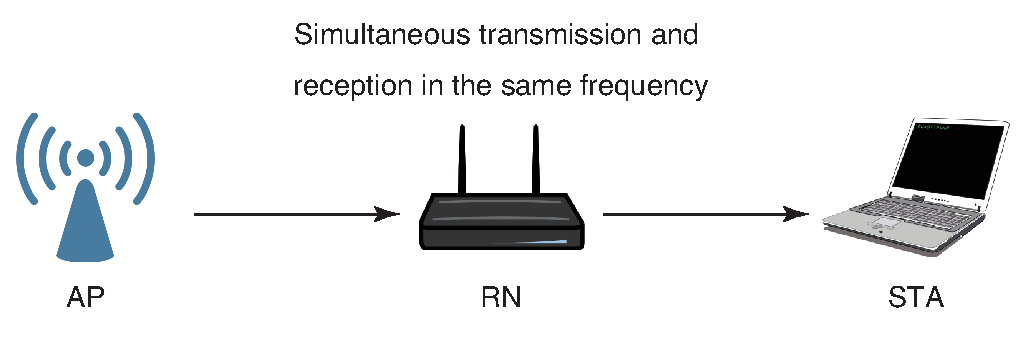
\epsfig{file=fig/model_relay.eps, scale=0.4}
		\caption{一方向全二重通信}
		\label{fig:topology}
	\end{figure}

\section{システムモデル}
	\begin{figure}[t]
		\centering
		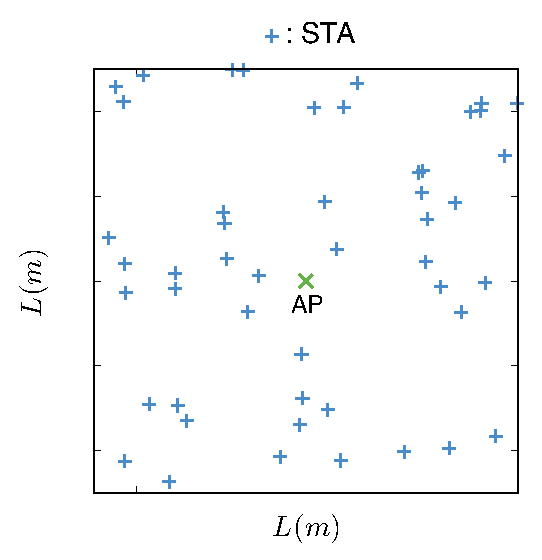
\epsfig{file=fig/pos.eps, scale=0.6}
		\caption{システムモデル}
		\label{fig:model}
	\end{figure}

	本稿で検討するシステムモデルを図\ref{fig:model}に示す.
	1台のAPが$L$四方の領域の中心に設置され,その周りに$N$台のSTAがランダムに配置されているとする.
	それらSTAのインデックス集合を$\mN=\{1,2,...,N\}$とする.
	この$N$台のSTAの中から,図\ref{fig:topology}のようにAPからの下り通信を受信するSTA $i$と,
	APへの上り通信を行うSTA $j$を選び出す.
	このとき,STAの組み合わせを$\sij$と表現し,$i,\ j \in \{0\}\cup \mN$であり,$i\neq j$とする.
	ただし,$i=0$のときは下り通信を伴わない上り通信のみの半二重通信であり,
	$j=0$のときは上り通信を伴わない下り通信のみの半二重通信であるとする.
	さらに,この$N$台のSTAの中に低遅延を要求するアプリケーションを用いているSTAが$n$台存在し,
	そのインデックス集合を${\mathcal D}\subset\mN$とする.
	ただし,低遅延を要求しないSTAのインデックス集合は${\overline {\mathcal D}}$と表し,
	${\mathcal D} \cup {\overline {\mathcal D}}=\mN,\ {\mathcal D} \cap {\overline {\mathcal D}}=\phi$とする.

\section{Probabilitsic-based adaptive full-duplex and half-duplex medium access control}
	\subsection{STAの組み合わせの決定手順}\label{sec:promac}
		本節では~\cite{promac}におけるSTAの組み合わせの決定手順について述べる.
		このMACプロトコルでは,APとSTA $i$,$j$の組み合わせで全二重通信が行われる確率$\pij$に基づいてSTA $i$,$j$が決定される.
		\par
		まず,全二重通信の組み合わせ
		\begin{equation}
			{\mathcal C}_{\rm full} \triangleq \{\sij : i,j\in{\mathcal N},\ i\neq j,\ r^{\sij}_{\rm d},\ r^{\sij}_{\rm u}>\epsilon\}
		\end{equation}
		に対して,上り下りそれぞれの実効スループット$\rd$,$\ru$を推定し,その合計を$\rij$とする.
		さらに,半二重通信の組み合わせ
		\begin{equation}
			{\mathcal C}_{\rm half} \triangleq \{\sij : i=0\ {\rm or}\ j=0,\ \rij >\epsilon\}
		\end{equation}
		に対しても実行スループット$\rij$を推定する.
		得られた$\rij$に基づいて以下の最適化問題を解き,確率$\pij$を得る.
		\begin{align}
			&{\mathcal P}_1: && {\rm max} \sum_{(i,\ j)\in{\mathcal C}} p^{(i,\ j)}r^{(i,\ j)} &&&&&& \label{eq:p1}\\
			&{\rm subject\ to} && \sum_{j\in\{j:(i,\ j)\in{\mathcal C}\}} p^{(i,\ j)} \geq \eta_{\rm d}^{(i)},\ \forall i\in {\mathcal N}  \\
			&&& \sum_{i\in\{i:(i,\ j)\in{\mathcal C}\}} p^{(i,\ j)} \geq \eta_{\rm u}^{(j)},\ \forall j\in {\mathcal N} \label{eq:pu}\\
			&&& \sum_{j\in\{j:(i,\ j)\in{\mathcal C}\}} p^{(i,\ j)}=1 \\
			&{\rm variables:} &&p^{(i,\ j)} \in {\mathbb R}_{\geq 0},\ \forall(i,\ j)\in {\mathcal C}
		\end{align}
		ただし,${\mathcal C} = {\mathcal C}_{\rm full} \cup {\mathcal C}_{\rm half}$である.
		$\eta_{\rm d}^{(i)}$はSTA $i$への下り通信のトラヒックに比例した値であり,
		STA $i$が下り通信の送信先となる確率$p_{\rm d}^{(i)}=\sum_{j\in\{j:(i,\ j)\in{\mathcal C}\}} p^{(i,\ j)}$
		の最低値を定める役割を果たす.
		同様に,$\eta_{\rm u}^{(j)}$はSTA $j$が持つ上り通信のトラヒックに比例した値であり,
		STA $j$が上り通信の送信権を得る確率$p_{\rm u}^{(i)}=\sum_{j\in\{i:(i,\ j)\in{\mathcal C}\}} p^{(i,\ j)}$
		の最低値を定める役割を果たす.
		また,以下の条件が満たされるとき必ず解が得られることが示されている.
		\begin{align}
			r_{\rm d}^{(i,\ 0)} &>\epsilon,\ \forall i\in\mN \\
			r_{\rm u}^{(0,\ j)} &>\epsilon,\ \forall j\in\mN \\
			\sum_{i\in\mN}\eta_{\rm d}^{(i)} + \sum_{j\in\mN}\eta_{\rm u}^{(j)} &=1 \label{eq:feasible}
		\end{align}
		なお,この最適化問題は最大でビーコンごとに解かれ,更新された確率$\pij$はビーコンフレームによってSTAに通知される.
		\par
		次に,得られた$\pij$を用いてSTA $i$,$j$を決定する方法を述べる.
		APは
		\begin{equation}
			p_{\rm d}^{(i)}= \sum_{j\in\{j:(i,\ j)\in{\mathcal C}\}}p^{(i,\ j)},\ \forall i \in \{0\}\cup{\mathcal N}
		\end{equation}
		によって各STAが下り通信の送信先となる確率$p_{\rm d}^{(i)}$を求め,この確率に従ってランダムに送信先STA $i$を選択する.
		さらに,
		\begin{equation}
			p_{\rm u}^{\sij} = P(j\ {\rm wins\ uplink|AP\ sends\ to}\ i)=\pij / p_{\rm d}^{(i)}
		\end{equation}
		によって得られた条件確率$p_{\rm u}^{\sij}$を用いて${\rm CW}^{\sij}_{\rm u}$を
		\begin{equation}
			{\rm CW}^{\sij}_{\rm u} = \lceil 1/p_{\rm u}^{(j)} \rceil
		\end{equation}
		と設定し,${\rm CW}^{\sij}_{\rm u}$をコンテンションウィンドウサイズとしたバックオフアルゴリズムによってSTA $j$が決まる.

	\subsection{問題点}
		前節で述べたように~\cite{promac}では,STA $i$,$j$の干渉が小さい組み合わせが選ばれやすい.
		図\ref{fig:numtx}にこのSTAの組み合わせの決定手順を再現したシミュレーションによって得られた各STAの上り通信送信回数を示す.
		結果からわかるように,一部のSTAが非常に選ばれやすいことがわかる,
		このことから,送信機会に関する公平性は低く,加えて,低遅延を要求するようなアプリケーションを利用しているSTAが存在する場合にも,
		その要求に応えることはできないという問題がある.
		本稿では,この2つの問題点に関して解決を図り,QoSの向上を目指す.

		\begin{figure}[t]
			\centering
			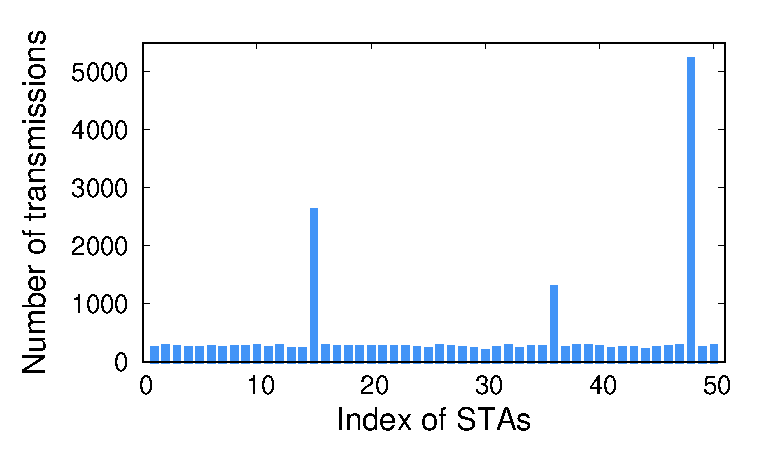
\epsfig{file=graph/numtx.eps, scale=0.6}
			\caption{STAの送信回数}
			\label{fig:numtx}
		\end{figure}

\section{提案方式}
\subsection{公平性の改善}\label{sec:fair}
	本節ではSTA間の送信機会の公平性を改善するための検討を行う.
	最初に述べたように既存のMACプロトコルでは干渉が小さい組み合わせが選ばれやすく,
	STA間の公平性が低下するという問題点がある.
	この問題を解決をするため以下のように,式\eqref{eq:p1}に待機時間$d^{(j)}$の項を評価関数に追加する.
	\begin{equation}
		{\mathcal P}_2: {\rm max} \sum_{(i,\ j)\in{\mathcal C}} p^{(i,\ j)}r^{(i,\ j)}(d^{(j)})^{\alpha} \label{eq:p2}
	\end{equation}
	待機時間$d^{(j)}$とはSTA $j$のバッファの先頭にフレームが到着してから現在時刻までの時間である.
	この待機時間の項を追加することで,待機時間が長いSTAを含んだ組み合わせが選ばれる確率が高くなり,
	送信機会を得られていないSTAほど送信機会を得やすくなる.
	また,待機時間は飽和トラヒックである限りは前回の送信時刻からの経過時間と同じであるため,
	新たに各STAの待機時間情報を収集する必要はなく,APが各STAごとに最新の送信時刻を記憶していれば,
	現在時刻との差として得られる.
	追加する項として各STAの平均送信間隔や送信回数そのものを選択しない理由は,
	両者はいずれも積算値であるため,瞬時性がなく,新たに追加されたSTAに対応できないためである.
	\par
	公平性の改善を行うと,公平性の改善を行わない場合に比べて比較的干渉の多いSTAの組み合わせが選ばれることが多くなり,
	システムスループットの低下が考えられる.
	そのため,公平性の改善とシステムスループットの低下のバランスを調整可能とするための重み$\alpha\geq 0$も導入している.
\subsection{低遅延を要求するSTAのQoSの向上}
	本節では,全体の公平性を改善した上で,さらに低遅延を要求するSTAのQoSを改善するための提案方式について述べる.
	低遅延を要求するSTAのQoSを向上させるためには,
	上り通信を行う確率$p_{\rm u}^{(j)}$を大きくし,送信機会を増加させればよい.
	これを実現するために,式\eqref{eq:pu}において$p_{\rm u}^{(j)}$の最低値を決定していた$\etau$を大きくすることを考える.
	具体的には,以下の式のように低遅延を要求していないSTAから送信確率を$x_j$だけ譲り受け,
	それを低遅延を要求するSTAで分け合うという方法をとる.
	\begin{align}
		{\hat \eta}_{\rm u}^{(j)} &= \etau -x_j > 0,\ \forall j \in {\overline {\mathcal D}} \label{eq:etadbar}\\
		{\hat \eta}_{\rm u}^{(j)} &= \etau + x_j, \ \forall j \in {\mathcal D} \label{eq:etad}\\
		\sum_{j\in{\overline {\mathcal D}}} x_j &= \sum_{j\in{\mathcal D}} x_j \label{eq:sub}
	\end{align}
	なお,式\eqref{eq:sub}は式\eqref{eq:feasible}を満たし可解性を失わないための条件である.
	これによって,低遅延を要求するSTAの送信機会が増加し送信間隔が短くなることで遅延時間が短縮されQoSが改善される.

\section{シミュレーション評価}
	本章では提案手法の効果をシミュレーションによって評価する.
	共通のシミュレーション諸元を表\ref{tab:param}に示す.
	MACプロトコルは~\cite{promac}に従い,上下通信ともに飽和トラヒックであるものとする.

	\begin{table}[t]
		\centering
		\caption{シミュレーション諸元}
		\label{tab:param}
		\begin{tabular}{cc} \hline
			領域の大きさ $L$ & 100\,m \\
			伝送速度 & シャノン容量 \\
			送信電力 & 15\,dBm \\
			雑音指数 & 10\,dB \\
			減衰定数 & 3 \\
			周波数帯 & 5\,GHz \\
			自己干渉キャンセル & 110\,dB \\ \hline
		\end{tabular}
	\end{table}

	\subsection{公平性の改善}
	図\ref{fig:fair}に$N=50$とした場合の各STAの上り通信送信回数を示す.
	図\ref{fig:numtx}と比較して,一部のSTAが極端に選ばれやすいという現象が改善されていることがわかる.
	次に,システムスループットと公平性の関係性を確認するため,
	図\ref{fig:thr_fair}にシステムスループットとSTA間の公平性を示す.
	ただし,いずれも10種のSTA配置の平均値であり,
	公平性の評価はJain's fairness index~\cite{jain}に各STAの送信回数を代入することで求めている.
	STA間の送信機会に関する公平性を大きく改善できたうえ,
	重み$\alpha$を変化させることで,公平性の改善とシステムスループット低下のバランスをシステムの要求に応じて変化させられることがわかる.
	また,この場合$\alpha=3$のときにスループットの低下が小さく,公平性が高くなっている.
	\par
	次に,このスループットの低下が小さく,公平性が高くなる$\alpha$の値がシミュレーション条件によってどのように変化するかを示す.
	図\ref{fig:chgparam}\subref{fig:chgtopology}にSTAの配置を変更した場合のシステムスループットとSTA間の公平性を示す.
	この場合,システムスループットの低下が小さく,STA間の公平性が高い$\alpha$の値は0.2程度である.
	さらに,図\ref{fig:chgparam}\subref{fig:chgnum}にSTA台数を$N=30$とした場合の結果を示す.
	この場合にも,$\alpha=0.2$あたりでバランスが良いことがわかる.
	いずれもスループットの値やfaieness indexの値は異なるが,概ね$\alpha$は0.2から0.3で公平性の改善とスループットの低下のバランスが良いことがわかる.

	\begin{figure}[t]
		\centering
		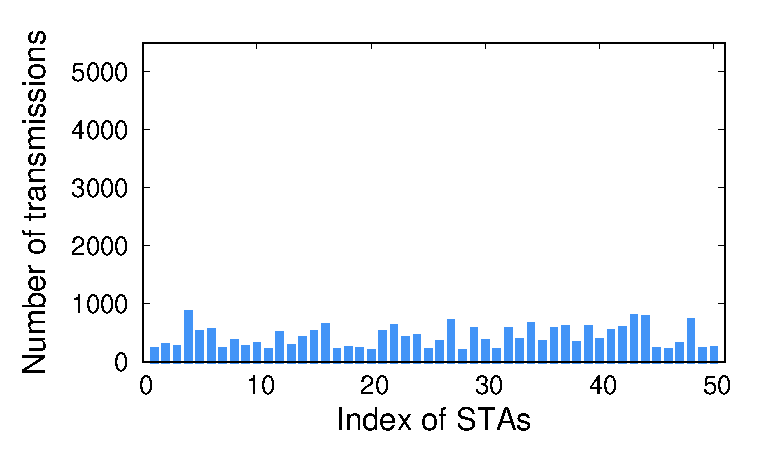
\epsfig{file=graph/numtxfair.eps, scale=0.6}
		\caption{STA間の送信機会に関する公平性の改善}
		\label{fig:fair}
	\end{figure}

	\begin{figure}[t]
		\centering
		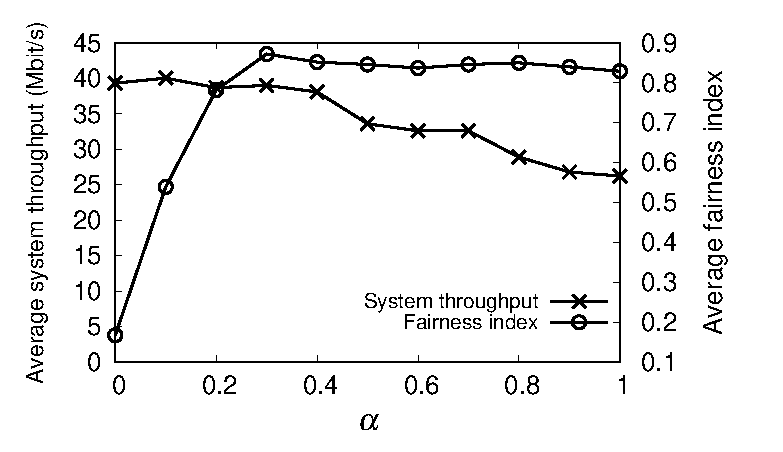
\epsfig{file=graph/thr_fair.eps, scale=0.6}
		\caption{STA間の送信機会に関する公平性の改善}
		\label{fig:thr_fair}
	\end{figure}

	\begin{figure}[t]
		\centering
		\subfloat[STAの配置を変更した場合]{
			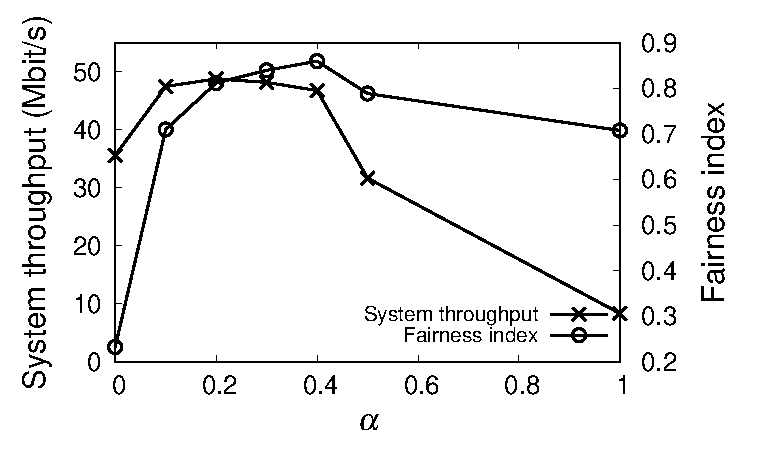
\epsfig{file=graph/chgtopology.eps, scale=0.6}
			\label{fig:chgtopology}
		}
		\\
		\subfloat[STA台数を$N=30$に変更した場合]{
			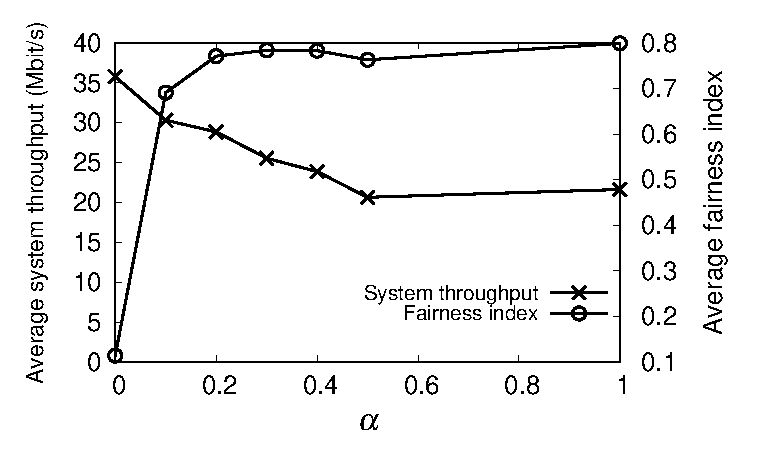
\epsfig{file=graph/chgnum.eps, scale=0.6}
			\label{fig:chgnum}
		}
		\caption{シミュレーション条件を変更した場合}
		\label{fig:chgparam}
	\end{figure}

	\subsection{低遅延を要求するSTAのQoSの向上}
	次に,低遅延を要求するSTAのQoS向上について評価を行う.
	本シミュレーションでは式\eqref{eq:etadbar}における$x_j$は
	低遅延を要求しない全STA共通の値$x_j=x,\ \forall j\in {\overline {\mathcal D}}$とし,
	式\eqref{eq:etad}における$x_j$も低遅延を要求する全STA共通の値$x_j=x|{\overline {\mathcal D}}|/|{\mathcal D}|,\ \forall j \in {\mathcal D}$とした.
	また,STA台数$N$は50台であり,$\alpha=0.3$である.
	\par
	まず最初に低遅延を要求するSTA台数を$n=5$,$x=0.05$とした場合に,それらの送信間隔が短縮されているかを確認する.
	低遅延を要求するSTAは${\mathcal D}=\{46,\ 47,\ 48,\ 49,\ 50\}$であるとする.
	図\ref{fig:inter}\subref{fig:interfair}に公平性のみを考慮した場合の,
	図\ref{fig:inter}\subref{fig:intereta}に低遅延を要求するSTAの送信機会を増加させた場合の各STAの平均送信間隔を示す.
	公平性のみを考慮した場合は全STA間の送信機会の公平性が高いことから,
	送信間隔のばらつきが少ないが,低遅延を要求するSTA 46から50の送信間隔も平均43\,msと長い.
	一方,アプリケーションの違いを考慮し,低遅延を要求するSTAの送信機会を増加させたところ,
	送信間隔を15\,msと1/3程度まで削減することができた.

	\begin{figure}[t]
		\centering
		\subfloat[公平性の改善のみを行った場合のSTAの平均送信間隔]{
			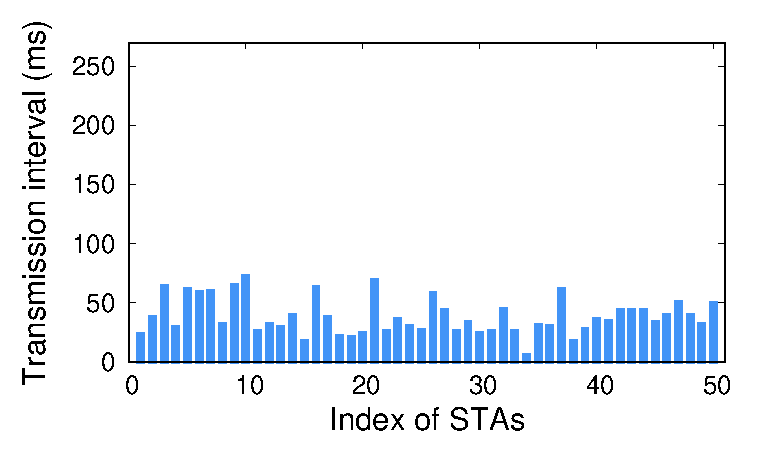
\epsfig{file=graph/interfair.eps, scale=0.6}
			\label{fig:interfair}
		}
		\\
		\subfloat[低遅延を要求するSTAの送信機会を増加させた場合のSTAの平均送信感覚]{
			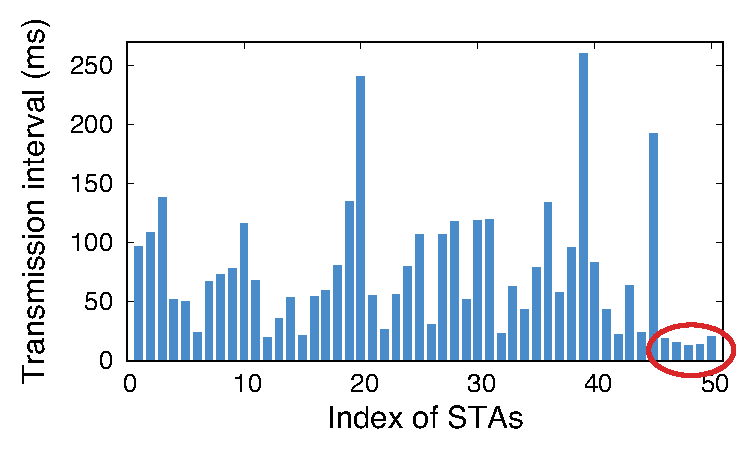
\epsfig{file=graph/intereta.eps, scale=0.6}
			\label{fig:intereta}
		}
		\caption{STAの平均送信間隔の比較}
		\label{fig:inter}
	\end{figure}

\section{まとめ}
本稿では,全二重通信無線LANの既存のMACプロトコルが持つSTA間の公平性の低さと
STAが利用しているアプリケーションの違いを考慮できていないといった問題について検討し,
それらを解決する手法を提案した.
各STAの待機時間を考慮することで,送信機会を得ることができていないSTAに送信機会を与えることで
STA間の公平性を大幅に改善し,さらに,重み$\alpha$によって公平性の改善とスループットの低下のバランスを調整できることを示した.
また,低遅延を要求するようなSTAの送信機会を増加させることでQoSの改善を行った.



\bibliographystyle{sieicej}
\bibliography{main2}

\end{document}
